\startchapter{Statistical Framework}
\label{chapter:stat}

This chapter presents the statistical framework which is used to search for evidence of new physics in the ATLAS collision data and, if no such evidence is found, establish the range of parameters over which the DH model is excluded by the search. Evidence of new physics would take the form of a statistically significant discrepancy between predicted yield distributions of SM background processes and collision data in the SRs. 

Owing to the presence of \ms-dependent peaks in the \minms distribution of the DH signal model in the SRs\footnote{See Section \ref{sec:minms} for details.}, the sensitivity of the search was found to be dramatically boosted by binning all data - MC simulated and ATLAS collision events - the SRs into several bins of \minms prior to performing the statistical analysis. Section \ref{sec:binning_strategy} presents the details of the binning strategy. Within each analysis region and bin, the statistical analysis is performed by fitting the predicted yields of background and signal processes to the ATLAS collision data with the aim of maximizing the profiled likelihood function presented in the following section. 

The computational construction and analysis of the profiled likelihood function is performed within the HistFitter \cite{Baak_2015} statistical analysis framework.

\section{Likelihood Function}
\label{sec:likelihood}

The likelihood function which lies at the heart of the statistical framework is a product of Poisson distributions of event counts in all regions and bins:

\begin{equation}
\label{eq:likelihood_func}
\begin{aligned}
L(\boldsymbol{n}, \boldsymbol{\theta}^0|\mu_\text{sig}, \boldsymbol{s}, \boldsymbol{\mu}, \boldsymbol{b}, \boldsymbol{\theta}) & = P_\text{SR} \times P_\text{CRs} \times C_\text{syst} \\
& = \prod_{i\in\text{SR bins}} P(n_{S,i}|\lambda_{S,i}(\mu_\text{sig}, \boldsymbol{\mu_i}, s_i, \boldsymbol{b_i}, \boldsymbol{\theta})) \times \\ 
&\phantom{xxx}\prod_{j \in \text{CRs}} P(n_j|\lambda_j(\mu_\text{sig}, \boldsymbol{\mu_j}, s_j, \boldsymbol{b_j}, \boldsymbol{\theta})) \times \\
&\phantom{xxx}C_\text{syst}(\boldsymbol{\theta}^0, \boldsymbol{\theta})
\end{aligned}
\end{equation}

where:

\begin{itemize}
    \item \(\boldsymbol{n}\in{n_{S,i}, n_j}\) is the set of all observed event counts in each region and bin.
    \item \(n_{S,i}\) and \(n_j\) are the number of observed events in the \(i^\text{th}\) bin of the SR and in the \(j^\text{th}\) CR, respectively.
    \item \(\boldsymbol{\mu}_i\) represents the normalization factors in each bin \(i\), which scale the \wjets and \ttbar backgrounds in all regions regions of the fit, with separate factors in the merged and resolved categories. The normalization factors are treated as unconstrained nuisance parameters (NPs) in the fit. They are initialized as 1 in the fit, with an uncertainty of \(\pm1\).  
    \item \(\boldsymbol{\theta}\) represents the set of NPs that parametrize all uncertainties associated with the MC simulated yields. For each normalization factor or uncertainty source \(i\), the corresponding nuisance parameter \(\theta_i\) continuously interpolates between the associated nominal and up/down shifts in predicted yield, as discussed in \Sect{4.4} of \Refn{~\cite{Baak_2015}}. For systematics sources, the NPs are normalized in the HistFitter framework such that \(\theta_i=0\) for the nominal yield, \(\theta=+1(-1)\) for the up (down) yield shift. NPs associated with statistical uncertainty of the predicted yields are instead normalized such that \(\theta=1\) represents the nominal yield in the given bin and \(\theta=1\pm1\sigma_\text{stat}/N\) represents \(\pm1\sigma\) yield shifts, where N and \(\sigma_\text{stat}\) are the expected yield in the bin and its statistical uncertainty, respectively. 
    \item The signal strength \(\mu_\text{sig}\) is an overall factor which scales the predicted yield of collision events produce by the DH signal model in all bins.
    \item \(C_\text{syst}(\boldsymbol{\theta}^0, \boldsymbol{\theta})\) is a composite function of Gaussian priors which is used to constrain the floating NPs \(\boldsymbol{\theta}\) in the fit based on their central values \(\boldsymbol{\theta^0}\) and uncertainties \(\boldsymbol{\kappa}\):

    \begin{equation}
    \label{eq:gaussian_np}
    C_\text{syst}(\boldsymbol{\theta}^0, \boldsymbol{\theta})= \prod_{j\in S} \frac{1}{\kappa\sqrt{2\pi}}e^{-\frac{1}{2}(\frac{\theta^0_j-\theta_j}{\kappa})^2}
    \end{equation}
    \noindent where \(S\) is the full set of uncertainties considered in the fit.
    
    \item The Poisson expectation functions \(\lambda_{S,i}(\mu_\text{sig}, \boldsymbol{\mu_i}, s_k, \boldsymbol{b_i}, \boldsymbol{\theta})\) and \(\lambda_j(\mu_\text{sig}, \boldsymbol{\mu_j}, s_j, \boldsymbol{b_j}, \boldsymbol{\theta})\), represent the total expected yield in each SR bin \(i\) and CR bin \(j\), respectively. 
\end{itemize}

\subsection{Poisson Expectation Formula}
\label{sec:poisson_exp}

Within a given SR bin or CR \(k\), the Poisson expectation function \(\lambda_k\) in Eq. \ref{eq:likelihood_func} is given by:
    
\begin{equation}
\label{eq:lambda}
        \lambda_k(\mu_\text{sig}, \boldsymbol{\mu_k}, s_k, \boldsymbol{b}_k, \boldsymbol{\theta}) = \mu_\text{sig}s_k\eta_{k, \text{sig}}(\boldsymbol{\theta}) + \sum\limits_{p\in{\text{\{SM bkg processes\}}}} \mu_{k,p} b_{k,p}\sigma_{k,p}(\boldsymbol{\theta})
\end{equation}
    
\noindent where \(s_k\) (\(b_{k,p}\)) is the yield of the signal process (SM background process \(p\)) predicted by MC simulation, as discussed in Section \ref{sec:MC_ATLAS}. \(\eta_{i,s}(\boldsymbol{\theta})\) is a scaling factor, nominally set to 1, which parametrizes the variations in expected yield induced by varying the NPs \(\boldsymbol{\theta}\) in the fit:

        \begin{equation}
            \label{eq:sigma}
            \eta_{k,p}(\boldsymbol{\theta}) = 1 + \sum_{s\in\text{all systematics}}I(\theta_s(k,p), \sigma_\text{down}(k,p), \sigma_\text{up}(k,p))
        \end{equation}

        where \(I(\theta_p, \sigma_\text{down}(i,s), \sigma_{up}(i,s))\) is continuous function of \(\theta_s(k,p)\) which interpolates\footnote{HistFitter employs a 6th-order polynomial to interpolate between  \(\sigma_\text{down}(i,s)\) and \(\sigma_\text{up}(k,p)\) a linear extrapolation beyond these extrema. See \Sect{4.1} of \Refn{~\cite{Cranmer:1456844}} for details.} the relative shift in predicted yield between the up and down extrema, \(\sigma_\text{up}(k,p)\) and \(\sigma_\text{down}(k,p)\), associated with varying the given uncertainty source by \(\pm1\sigma\). 

\subsection{Nuisance Parameter Nomenclature and Correlations}

Many of the NPs which appear in the likelihood function are correlated between bins, categories, and/or processes. For example, if a given NP is correlated between all bins in the fit, the value of the NP will be the same within all bins: \(\theta_s(k, p) \rightarrow \theta_s(p)\). The names given to NPs in the HistFitter framework reflect the presence of any such correlations by omitting the correlated parameter in the NP name. Taking the above example of an NP which is correlated between all bins, this correlation will be reflected by the omission of any bin number specification (eg \verb|_bin1|) 

The background normalization factors \(\boldsymbol{\mu}\) and uncertainty-related NPs \(\boldsymbol{\theta}\) are broken down as follows:

\begin{equation}
\label{eq:norm_factor_breakdown}
\boldsymbol{\mu}\in\{\mu_\text{\wjets, merged}, \mu_\text{\wjets, resolved}, \mu_\text{\ttbar, merged}, \mu_\text{\ttbar, resolved}\}
\end{equation}

\noindent and

\begin{equation}
\label{eq:norm_factor_breakdown}
\boldsymbol{\theta}\in\{\boldsymbol{\theta}_\text{statistical}, \boldsymbol{\theta}_\text{sys, experimental}, \boldsymbol{\theta}_\text{sys, theory}\}
\end{equation}

Table \ref{tab:np_naming} summarizes the correlations present for each type of NP, and the scheme used by HistFitter to assign names to each.

\begin{table}
\centering
\caption{Summary of correlations between nuisance parameters in the likelihood function}
\label{tab:np_naming}
%\begin{tabular}{l p{6cm} l l }
\footnotesize{
\begin{tabular}{p{2.5cm} p{4cm} p{4cm} p{3.5cm} }
\toprule
\textbf{NP Type} & \textbf{Description} & \textbf{Correlation Info} & \textbf{Naming Scheme} \\
\midrule
\midrule
\(-\) \(\mu_\text{\wjets, mgd}\) \newline \(-\) \(\mu_\text{\wjets, res}\) \newline \(-\) \(\mu_\text{\ttbar, mgd}\) \newline \(-\) \(\mu_\text{\ttbar, res}\) & Normalization factor which scales the \wjets (or \ttbar) background in all analysis regions and bins of the merged (resolved) category. & Correlated between all analysis regions and bins for the \wjets (or \ttbar) background in the merged (resolved) category. Not correlated between processes. & \(-\) \(\mu\){\uscore}Wjets{\uscore}mgd \newline \(-\) \(\mu\){\uscore}Wjets{\uscore}res \newline \(-\) \(\mu\){\uscore}ttbar{\uscore}mgd \newline \(-\) \(\mu\){\uscore}ttbar{\uscore}res \\
\midrule
\(\boldsymbol{\theta}_\text{statistical}\) & NPs which parameterize the statistical uncertainty associated with the predicted yield in each region and bin from MC simulation. & Correlated between all processes. Not correlated between regions or bins.  & \(\gamma\){\uscore}\{region\}{\uscore}\{category\}{\uscore}\newline\{bin type\}{\uscore}bin{\uscore}\newline\{bin index\} \\
\midrule
\(\boldsymbol{\theta}_\text{sys, experimental}\) & NPs which parameterize systematic uncertainties from experimental sources. & Correlated between all processes, regions and bins.  & \(\alpha\){\uscore}\{uncertainty source\} \\
\midrule
\(\boldsymbol{\theta}_\text{sys, theory}\) & NPs which parameterize systematic uncertainties for each process from theoretical sources. & Correlated between all regions and bins. Not correlated between processes.  & \(\alpha\){\uscore}{process}{\uscore}\newline\{uncertainty source\} \\
\bottomrule
\end{tabular}}
\end{table}


\section{Binning Strategy}
\label{sec:binning_strategy}

As shown in Figure \ref{fig:minms_shape_discrimination}, the \minms variable presented in Section \ref{sec:minms} has a \ms-dependent peaked distribution which for most \ms values is distinct in shape from the distribution of SM background processes. This shape discrimination between the signal and background processes is exploited when performing the likelihood fit by binning the MC simulated events and collision data into several \minms bins. 

\begin{figure}[htbp]
  \centering
    \begin{subfigure}[t]{0.48\textwidth}
    \centering
     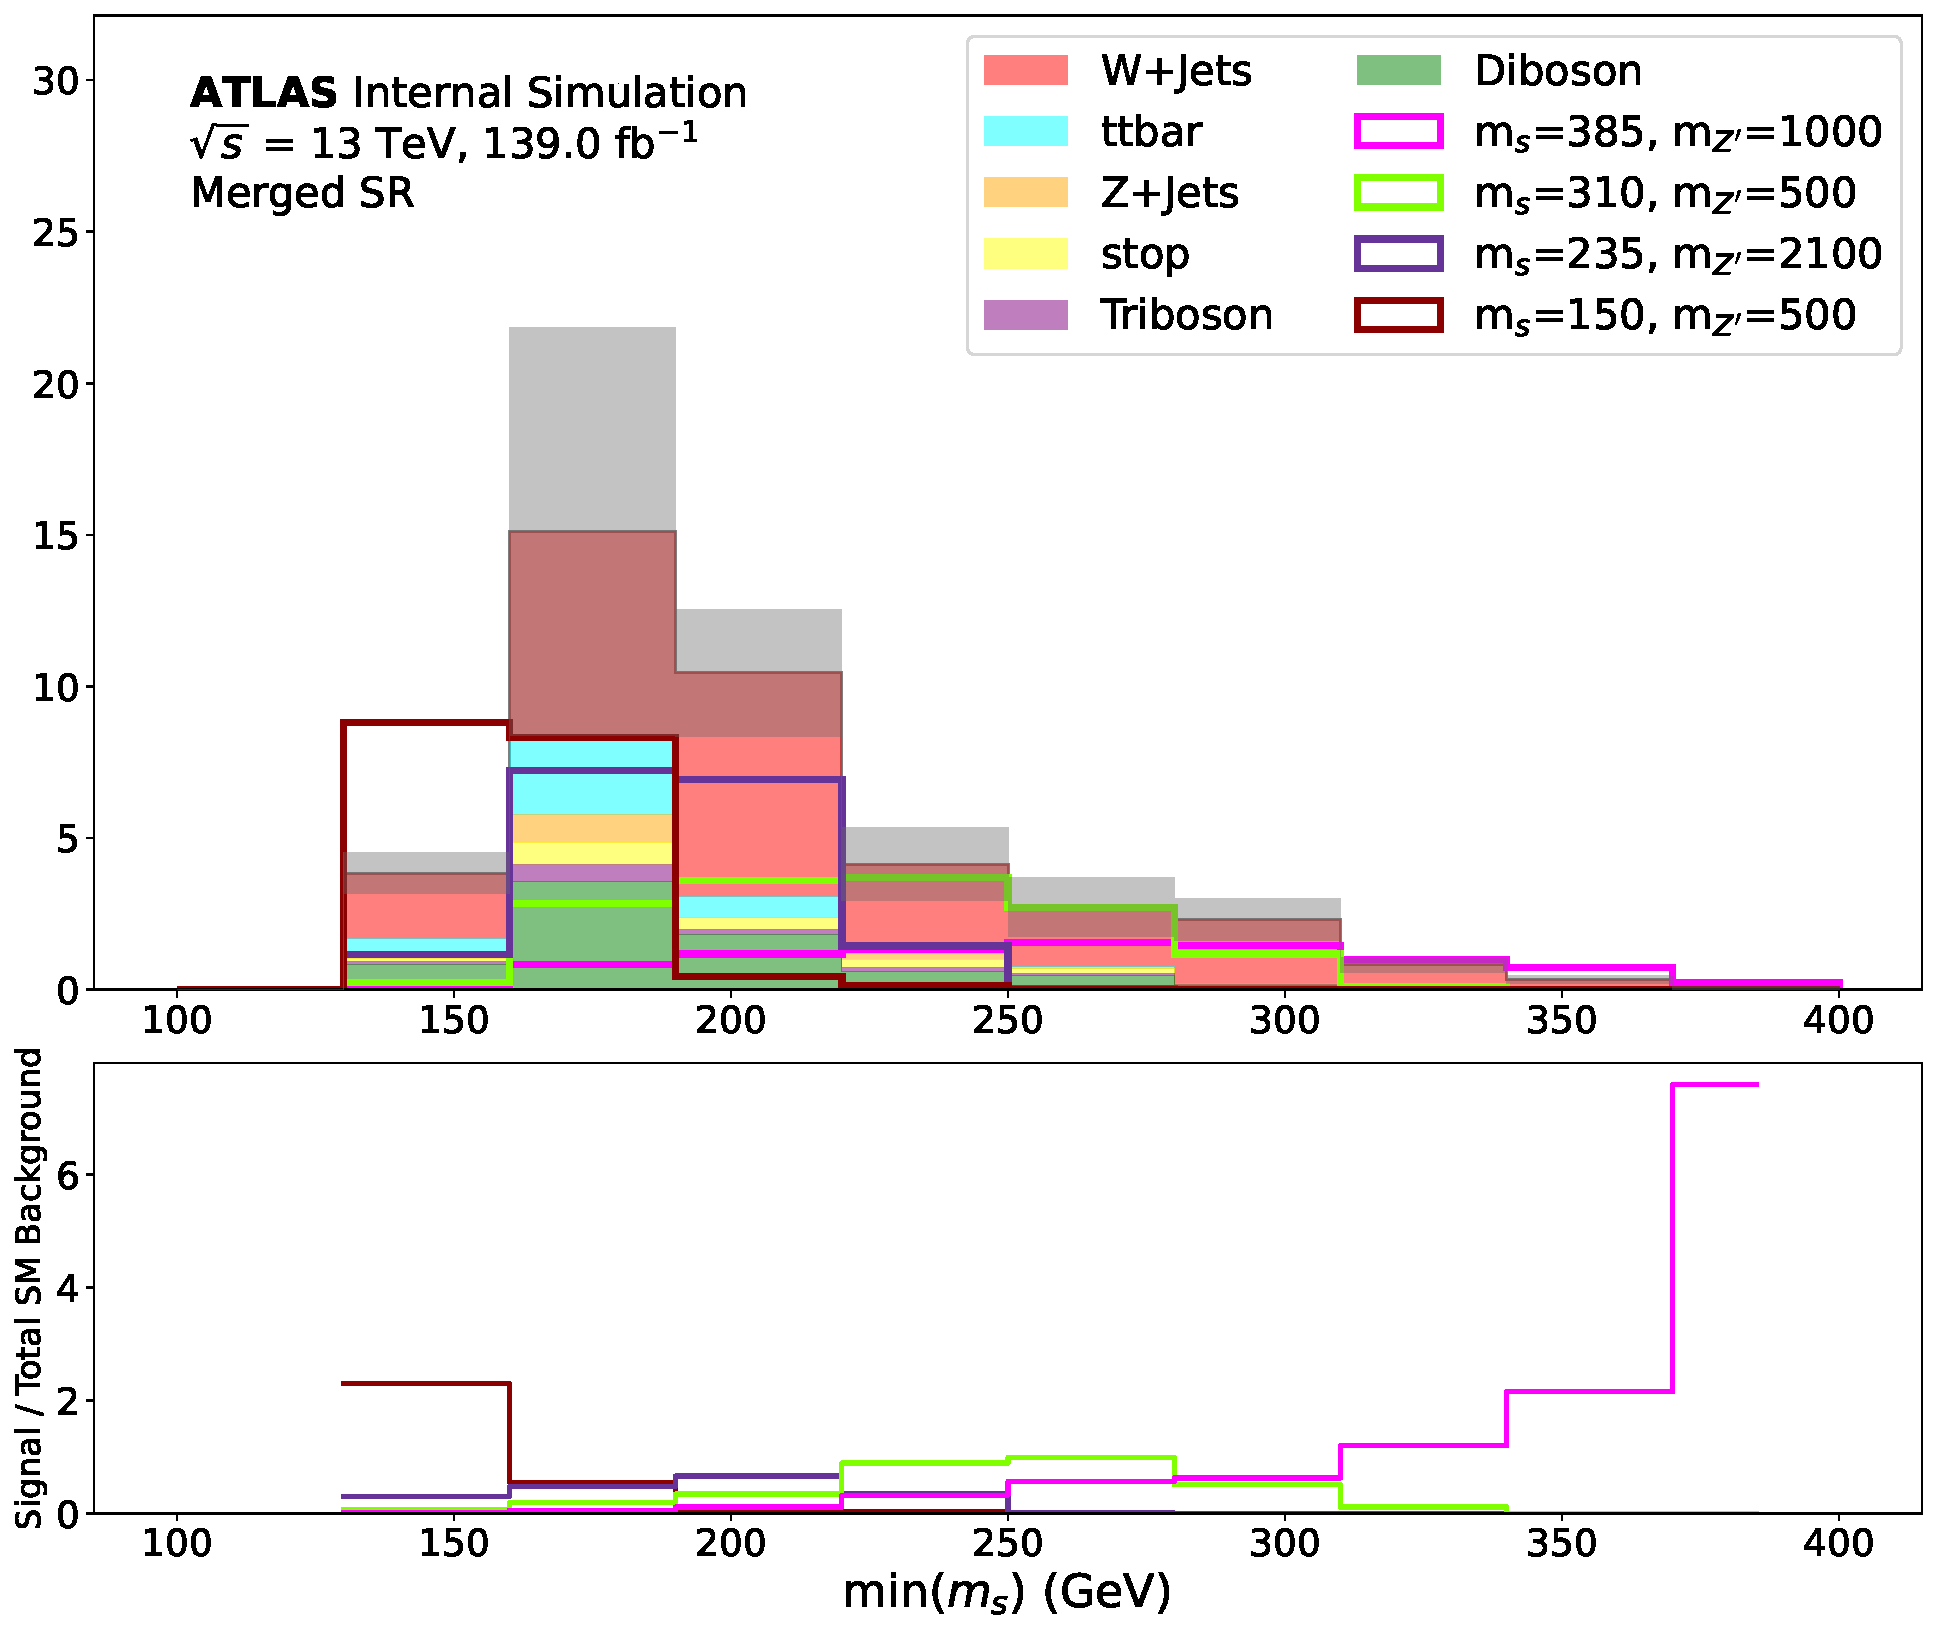
\includegraphics[width = 0.99\textwidth]{Figures/7/SR1L_Merged/TARJets10_minmS_mgd.pdf}
    \caption{Merged SR}
    \end{subfigure}
    \begin{subfigure}[t]{0.48\textwidth}
    \centering
     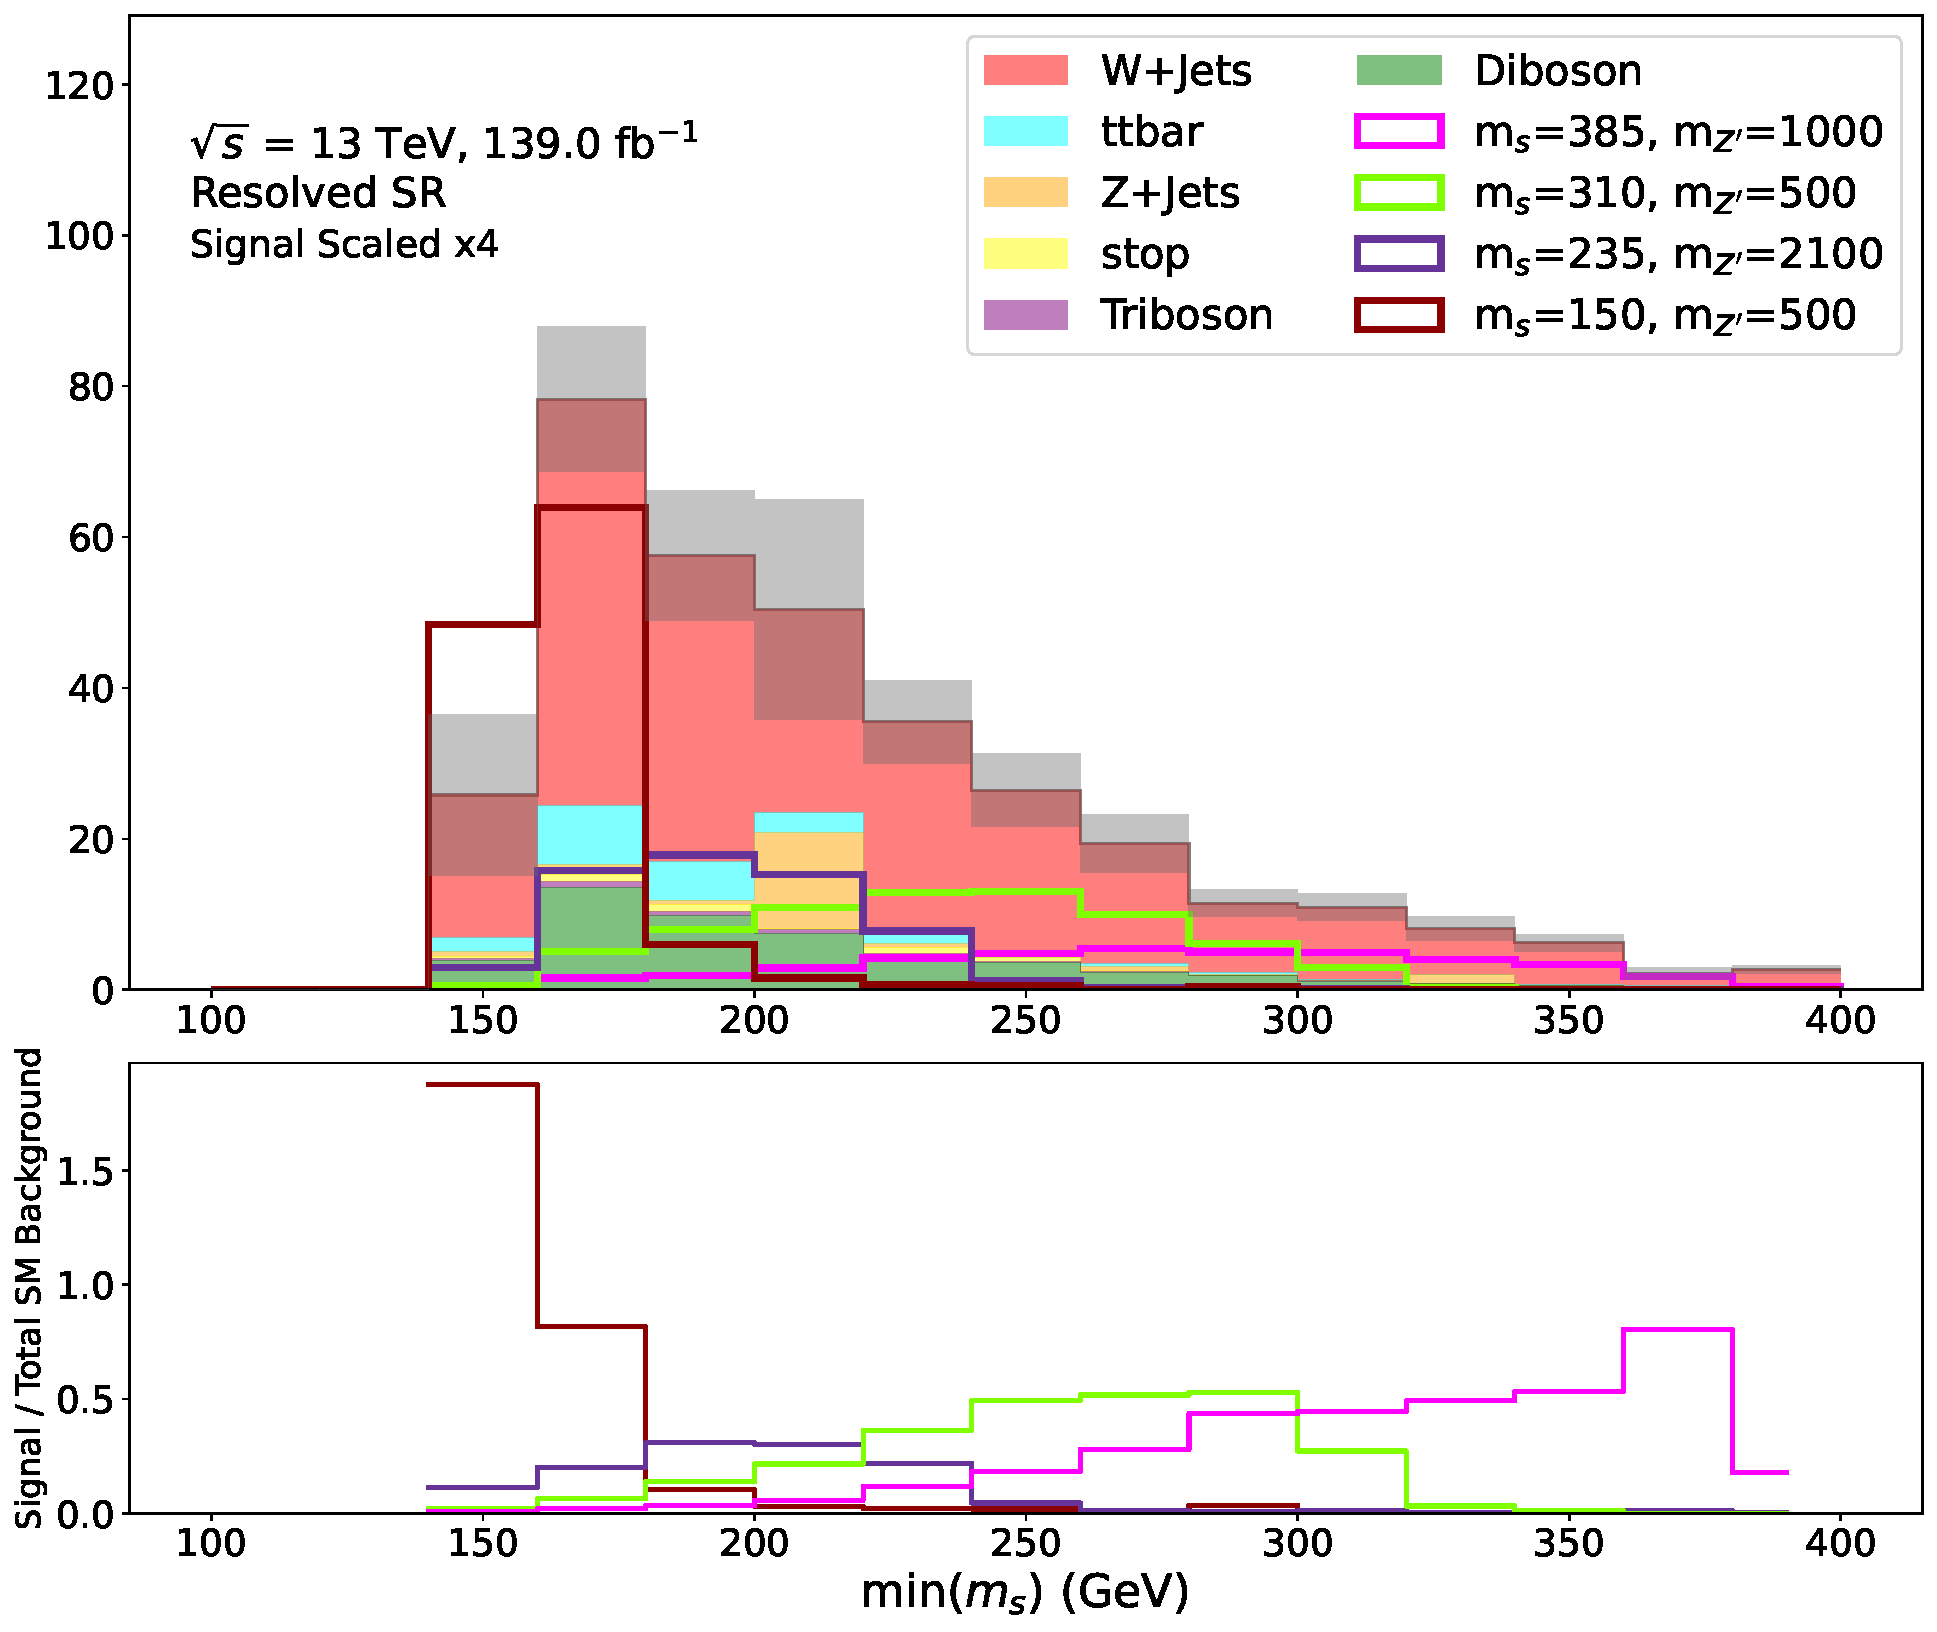
\includegraphics[width = 0.99\textwidth]{Figures/7/SR1L_Resolved/TARJets10_minmS_res.pdf}
     \caption{Resolved SR}
    \end{subfigure}
    \caption{Predicted yield of SM background (stacked filled) DH signal (unfilled) processes at several mass points in the merged (left) and resolved (right) SRs, binned in \minms. The lower panel shows the ratio of yields predicted for the DH signal process over the sum of MC background processes. Grey bands show the statistical uncertainty of the background estimate.}
   \label{fig:minms_shape_discrimination}
\end{figure}


The exact placement of bin edges in \minms used when performing the fit was optimized with the aim of maximizing the projected exclusion of the DH model for a background-only hypothesis using the limit-setting strategy presented in Section zzz. Distributions of \minms are shown with the optimized binning in Figure \ref{fig:minms_binning}. In the merged SR, binning the data into four \minms bins with non-equidistant bin edges was found to provide maximal sensitivity. In the resolved SR, binning into five \minms bins was found to be optimal, and equidistant bin edges are used, as no appreciable sensitivity improvements were found for non-equidistant binning.

\begin{figure}[htbp]
  \centering
    \begin{subfigure}[t]{0.48\textwidth}
    \centering
     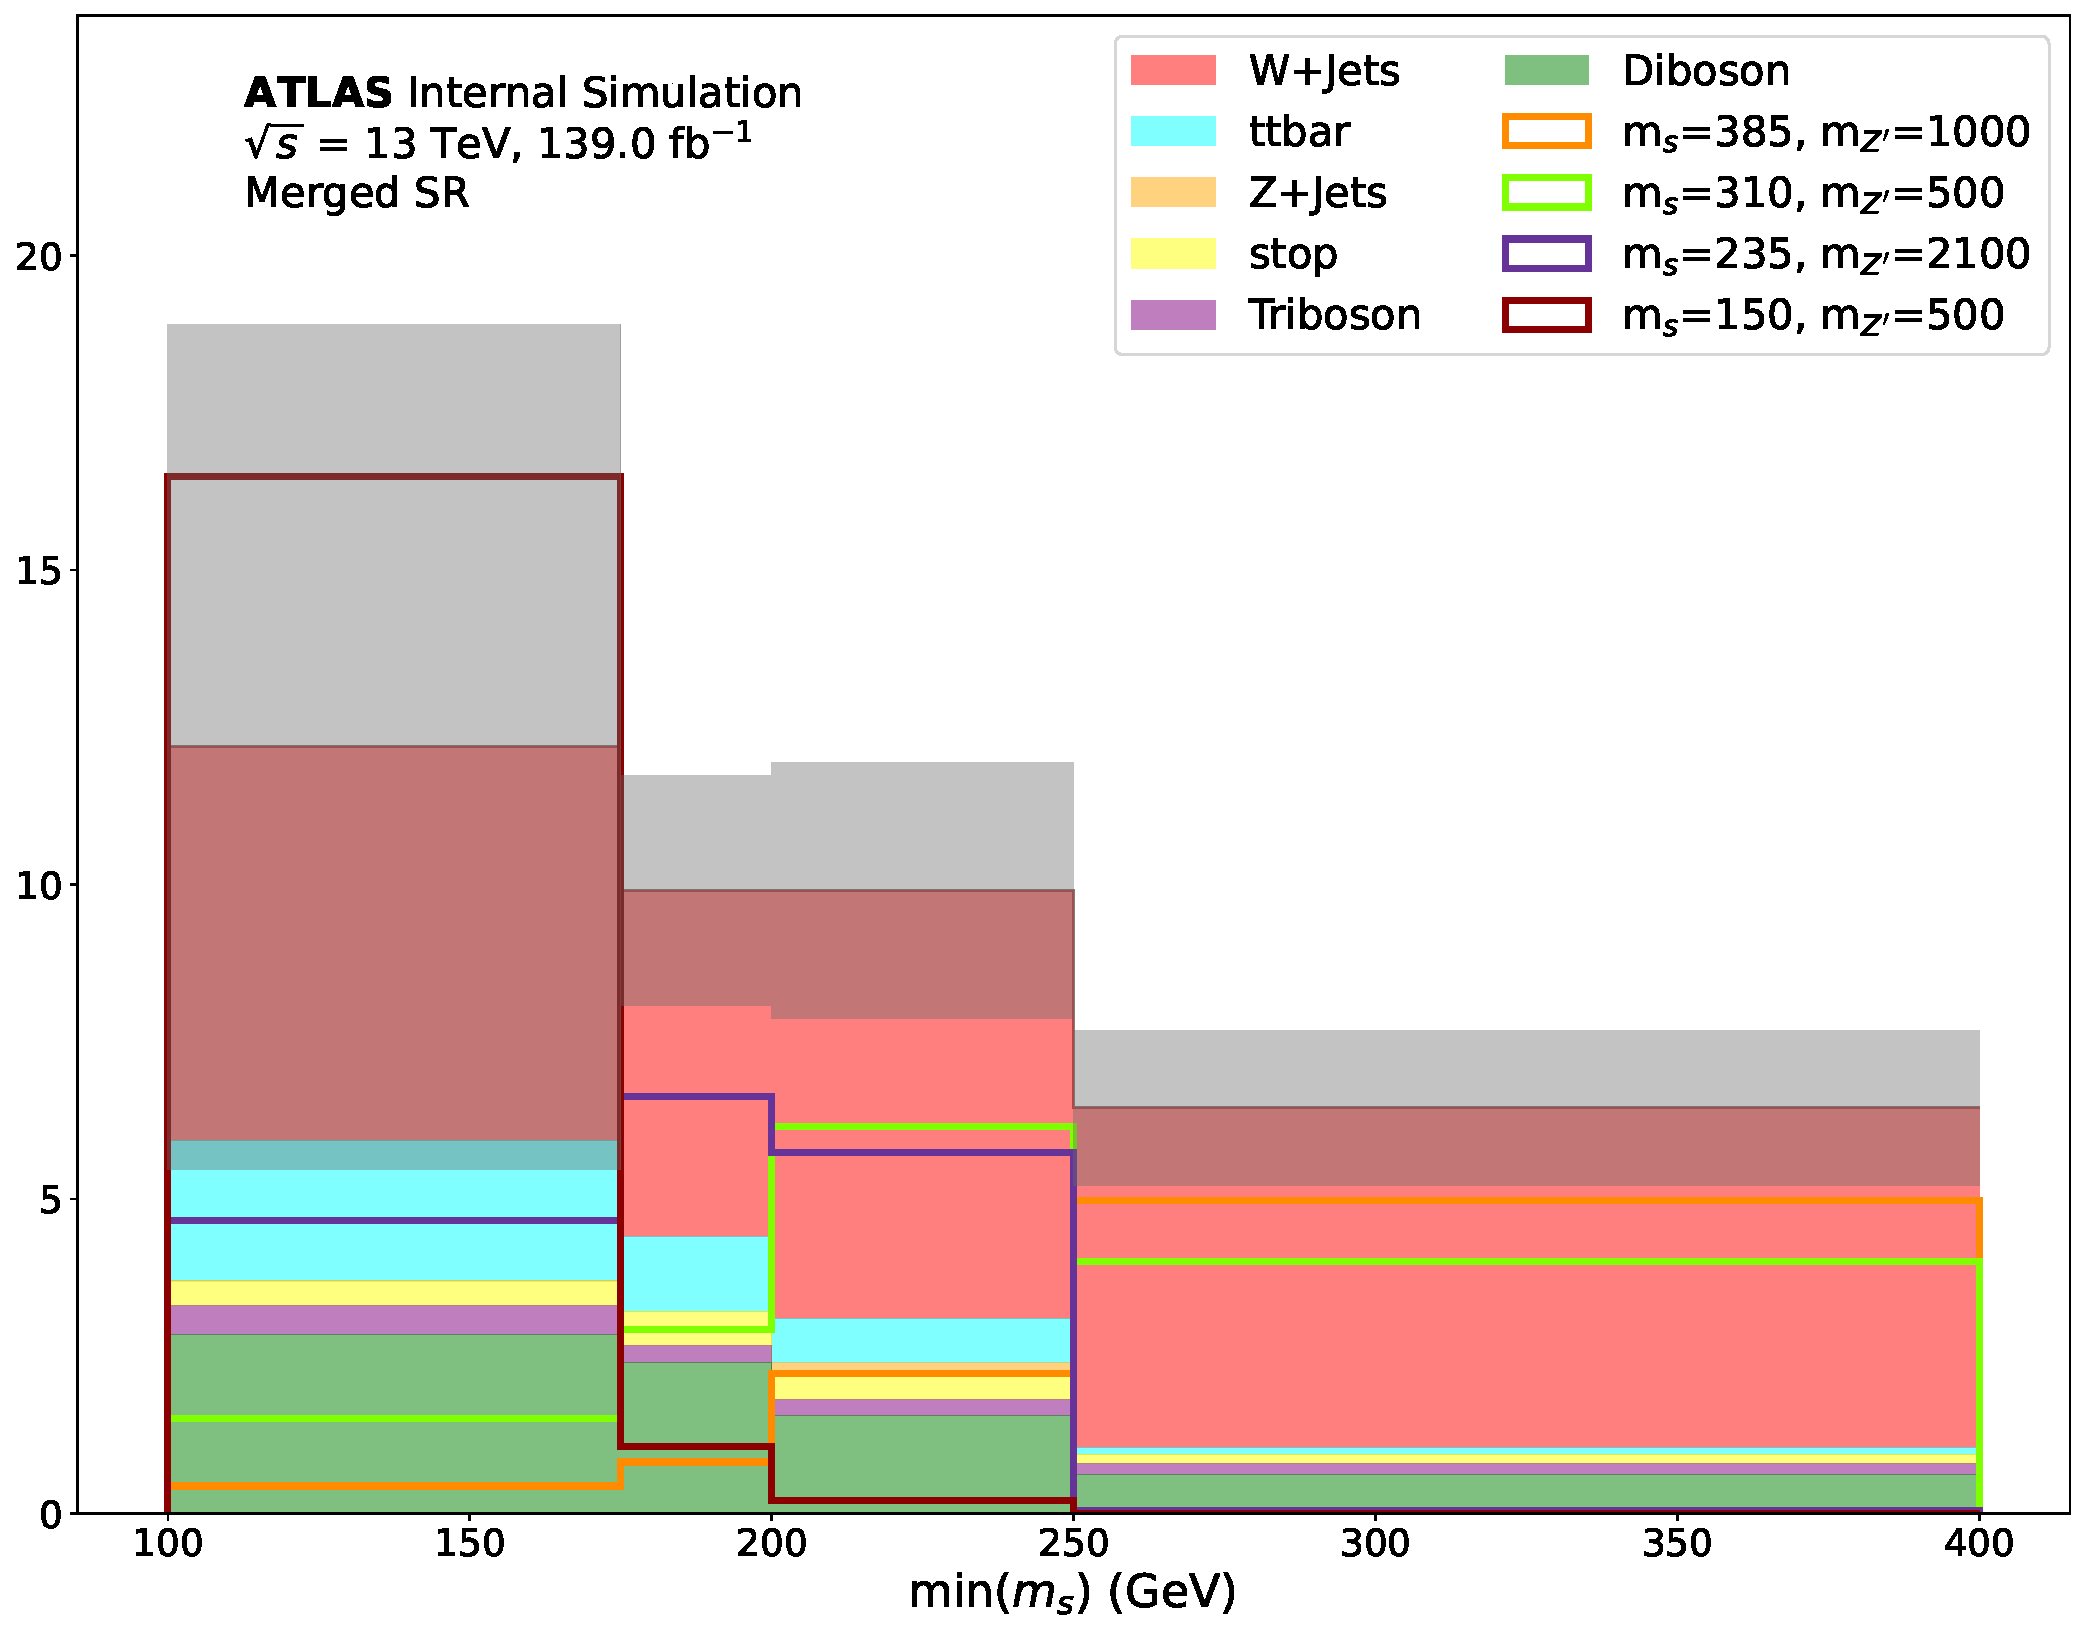
\includegraphics[width = 0.99\textwidth]{Figures/7/SR1L_Merged_fit/TARJets10_minmS_mgd.pdf}
    \caption{Merged SR}
    \end{subfigure}
    \begin{subfigure}[t]{0.48\textwidth}
    \centering
     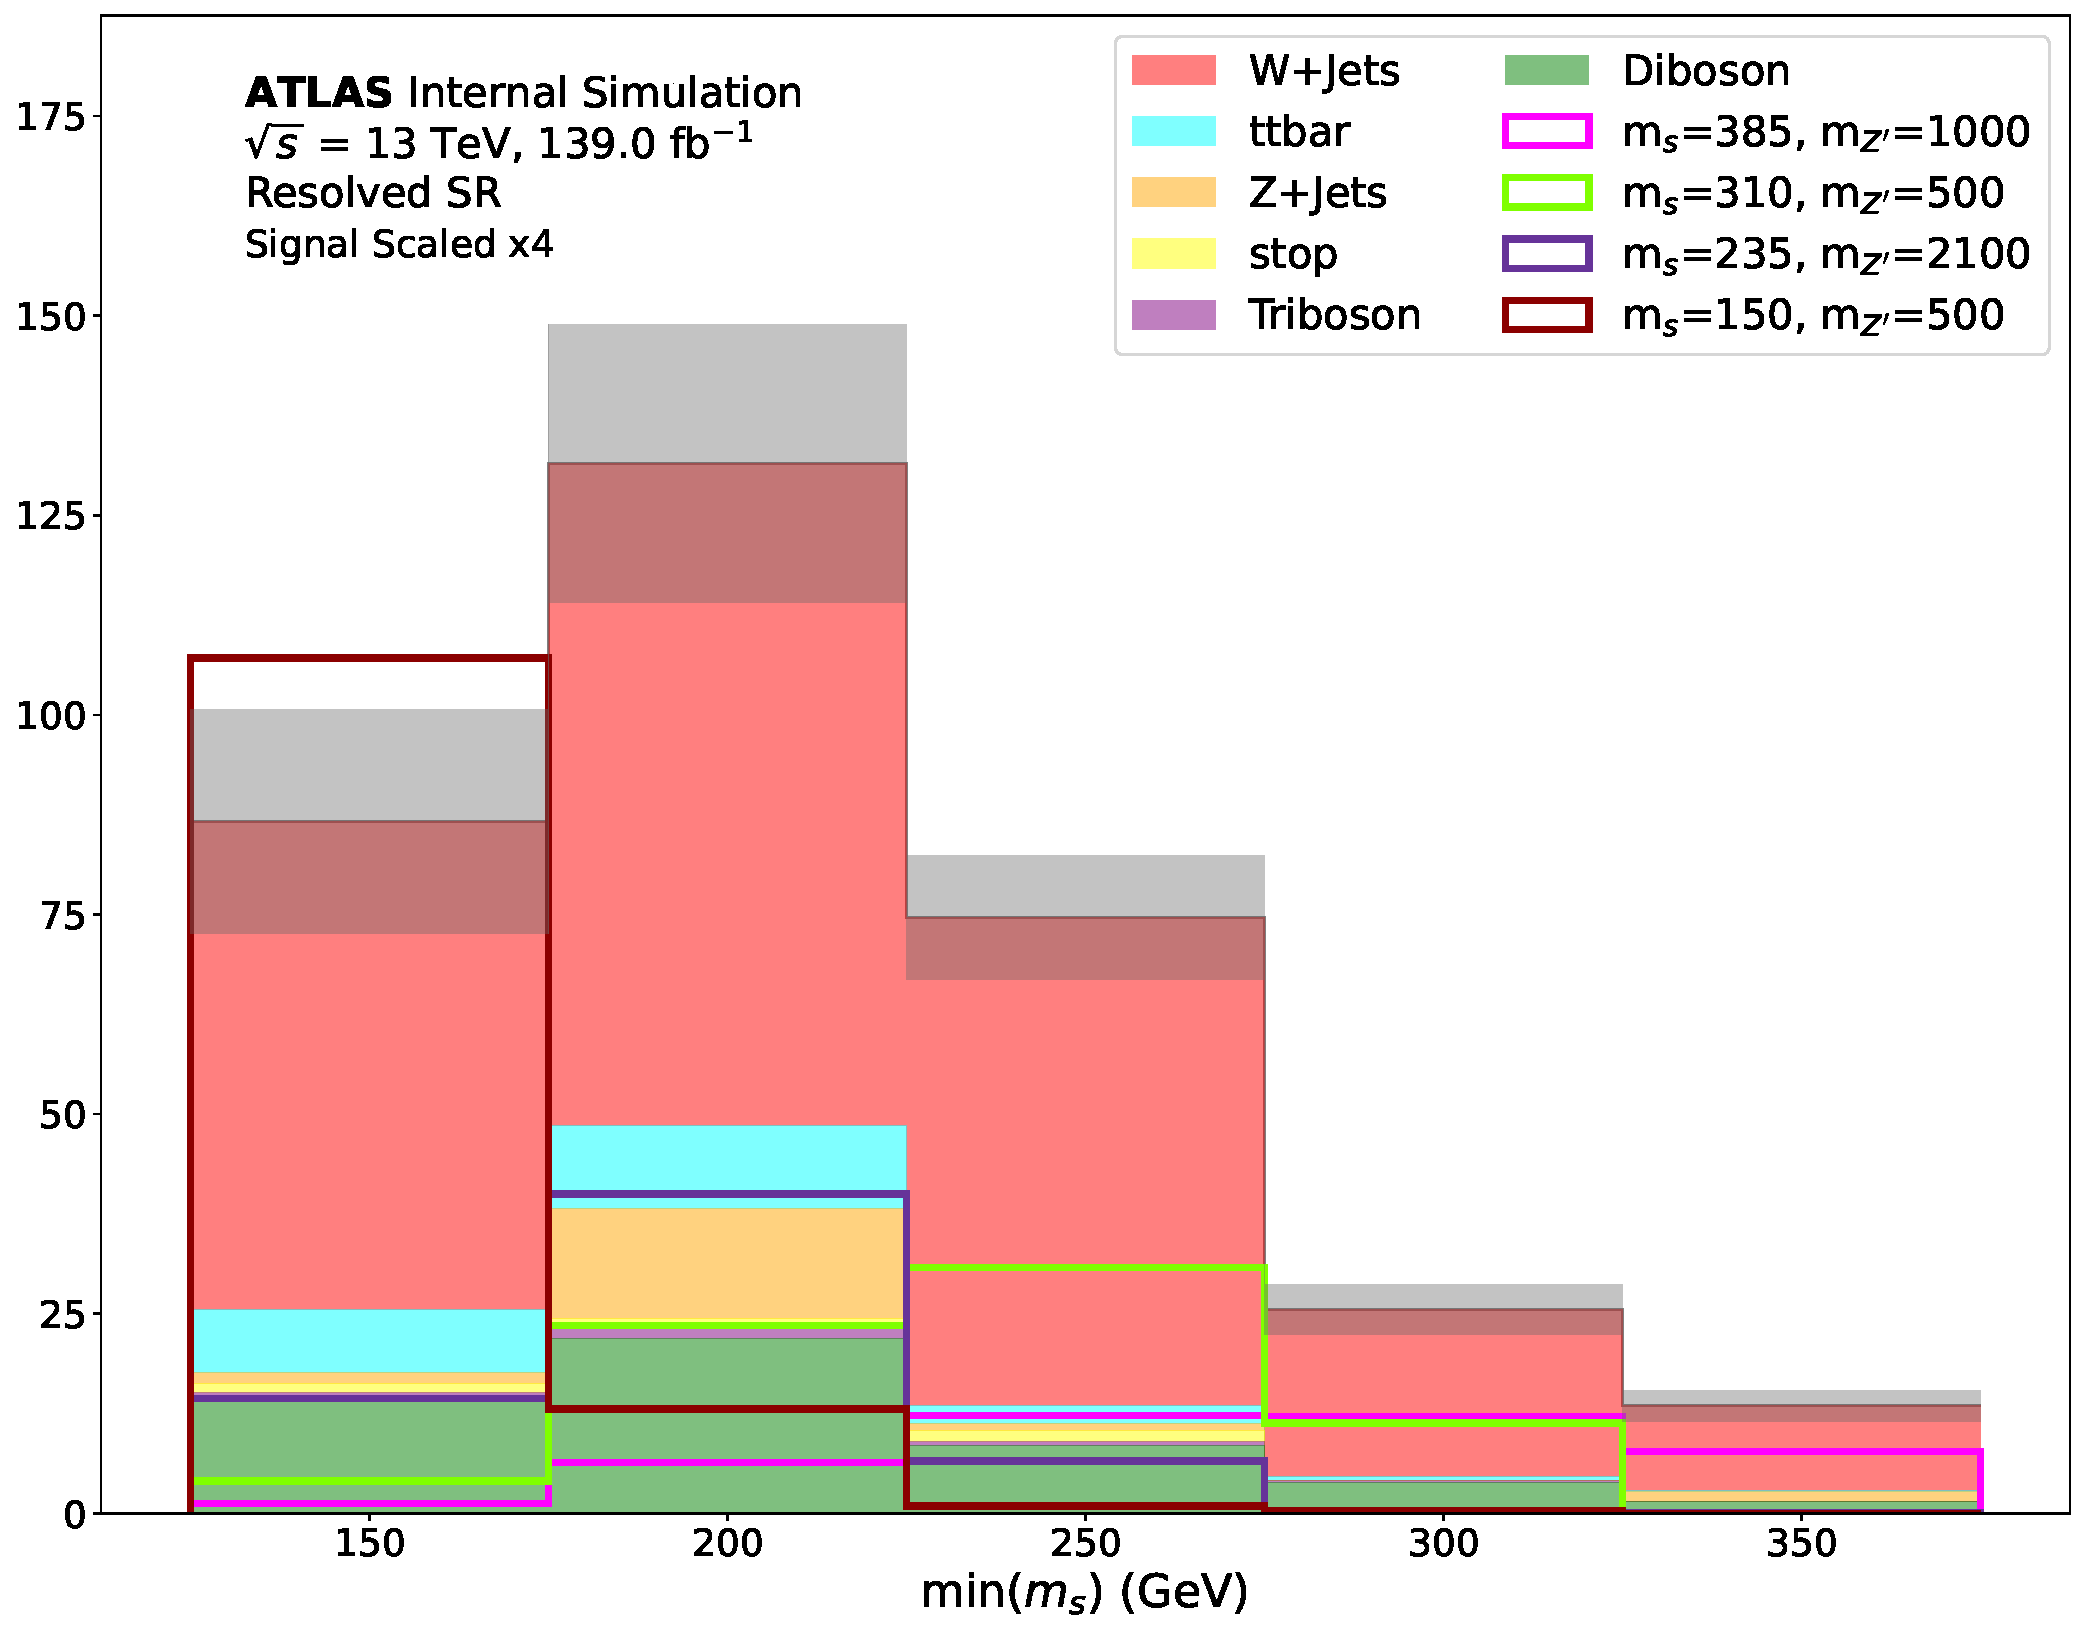
\includegraphics[width = 0.99\textwidth]{Figures/7/SR1L_Resolved_fit/TARJets10_minmS_res.pdf}
     \caption{Resolved SR}
    \end{subfigure}
    \caption{Predicted yield of SM background (stacked filled) DH signal (unfilled) processes at several mass points in the merged (left) and resolved (right) SRs, binned in \minms with the optimized bin edges. The lower panel shows the ratio of yields predicted for the DH signal process over the sum of MC background processes. Grey bands show the statistical uncertainty of the background estimate.}
   \label{fig:minms_binning}
\end{figure}

The CRs are left unbinned in the fit in order to provide constraints on the overall yield of the \wjets and \ttbar processes in each kinematic category. Table \ref{tab:statisticalevaluation_regions} summarizes the binning strategy in all analysis regions.

\begin{table}[ht]
\centering
\footnotesize{
    \caption{Binning used in the regions entering the statistical analysis.}
    \label{tab:statisticalevaluation_regions}
    \begin{tabular}{l ll}
    \toprule
    \textbf{Region}         &  \textbf{Binning in Merged Category} & \textbf{Binning in Resolved Category} \\
    \midrule
    \midrule
    \multirow{2}{*}{SR} & 4 non-equidistant bins in \(m_s\) & 5 equidistant bins in \(m_{s}\)  \\
    					     & bin edges: [125, 165, 190, 225, 375] \GeV & bin edges: [125, 175, 225, 275, 325, 375] \GeV \\
    \midrule   					   
    \wjets CR & none & none \\
    \midrule    
    \ttbar CR & none  & none \\ 
    \bottomrule
    \end{tabular}}
\end{table}

\subsection{Fit Setup}
\label{sec:fit_setup}


\subsection{Background-only Fit and Signal Region Extrapolation}
\label{sec:extrapolation}

To 

\subsection{Exclusion Hypothesis Test}
\label{ap:hypo_test}



\begin{itemize}
\item Presentation of how normalization factors for the \wjets and \ttbar backgrounds are constrained in the CRs using a background-only fit and extrapolated to the SRs. 
\item Discussion of the evaluation of transfer factor systematics for the \wjets and \ttbar backgrounds to account for the above normalization constraint and extrapolation procedure.
\item Presentation of the discovery test to be done after unblinding $\rightarrow$ check if any fits for signal strength with unblinded data produce a statistically significant inconsistency with 0.
\item Presentation of the profiled log-likelihood ratio $q_{\mu_\text{sig}}$, and description of how $q_{\mu_\text{sig}}$ is used to calculate a p-value for the exclusion hypothesis test (in case no significant excess found in the discovery test).
\item Discussion of the use of the asymptotic formula to avoid the need to throw random pseudo-experiments when evaluating the p-value, and its regime of validity ($>\mathcal{O}(5)$ events per bin).
\item Brief discussion of the CLs method for limit setting.
\item Description of how the limits are presented in the \ms vs. $m_{Z'}$ plane.
\end{itemize}
